\section{UDP Pinger}
Socket programming (UDP/IP)을 통해서 Ping application을 만들었다.

\subsection{Code}
\vspace{-4mm}
\begin{listing}[h!]
\inputminted[framerule = 1pt,framesep = 2mm , frame = lines, fontsize=\footnotesize]{python}{./code/week09/03/UDP_Pinger_Server.py}
\caption{\footnotesize Experiment 3, UDP Pinger Server.py}
\end{listing}
\clearpage

\vspace{-4mm}
\begin{listing}[h!]
\inputminted[framerule = 1pt,framesep = 2mm , frame = lines, fontsize=\footnotesize]{python}{./code/week09/03/UDP_Pinger_Client.py}
\caption{\footnotesize Experiment 3, UDP Pinger Client.py}
\end{listing}
\clearpage

\subsection{Process Analysis}
\begin{enumerate}
    \item UDP/IP Server/Client socket 생성(socket) 및 Server의 IP 주소와 Port 번호 설정(bind)
    \item Client가 Server에게 ping 메세지 송신(sendto/recvfrom)
    \item Server는 Client에게 response 메세지 송신(sendto/recvfrom), 일정 확률로 packet loss가 발생해 ping response를 보내지 않는다.
    \item Client가 ping 메세지와 response 메세지 사이의 시간 차이로 RTT 계산, 3.5초 동안 ping response가 없으면 time out으로 처리
    \item 2~4를 10번 반복한다.
    \item Client socket close
\end{enumerate}

\subsection{Experiment Result}
Terminal에 Server를 실행했다. \\
\vspace{-4mm}
\begin{figure}[!h]\centering 
	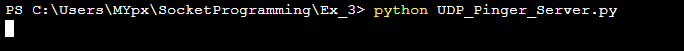
\includegraphics[width=.99\textwidth]{image/week09/3-1.png}
	\caption{\footnotesize
	Server Terminal}
	\vspace{-10pt}
\end{figure}

Terminal에 Client를 실행했다. 10번의 ping 메세지를 보내 6개의 reply를 받았고, 각 ping의 RTT를 계산했다. 나머지 4개의 ping은 response 메세지를 받지 못해 Request time out으로 처리됐다. \\
\vspace{-4mm}
\begin{figure}[!h]\centering 
	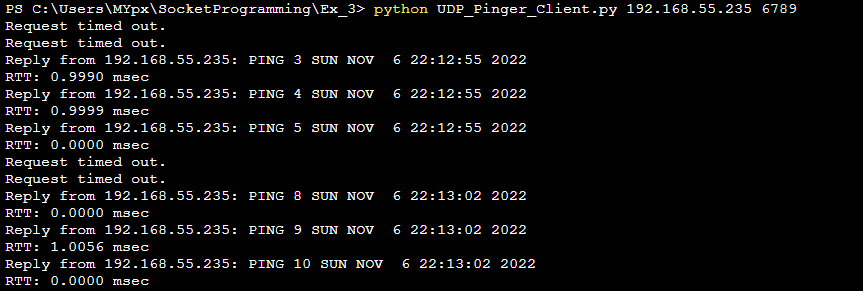
\includegraphics[width=.99\textwidth]{image/week09/3-2.png}
	\caption{\footnotesize
	Client Terminal}
	\vspace{-10pt}
\end{figure}

\clearpage
